\documentclass[12pt,fleqn,unicode]{article}
\usepackage{Diplo}
\usepackage{tikz}
\usepackage{mathtools}
\usetikzlibrary{shapes,arrows,shadows}
% \usepackage{subcaption}
\usepackage{subfig}

% \usepackage{graphicx}
%\usepackage{caption}
%\usepackage{subcaption}
%\usepackage[cp1251]{inputenc}
%\usepackage{amssymb,amsmath}
%\usepackage[russian]{babel}
%\usepackage{array}
%\usepackage[ruled,section]{algorithm}
%\usepackage[noend]{algorithmic}
%\usepackage[all]{xy}
%\usepackage{graphicx}
%\usepackage{indentfirst}
% \usepackage{bigstrut}
% \usepackage{float}
% \DeclareMathOperator*{\argmax}{arg\,max}

%\clubpenalty=10000
%\widowpenalty=10000
%% для больших плавающих иллюстраций
%\renewcommand\topfraction{1.0}
%\renewcommand\textfraction{0.0}
%\renewcommand\floatpagefraction{0.01} % float-страниц быть вообще не должно - это чтобы их лучше видеть ;)
% Воронцов
% \newcommand\brop[1]{#1\discretionary{}{\hbox{$\mathsurround=0pt #1$}}{}}
\newcommand{\tsum}{\mathop{\textstyle\sum}\limits}
\renewcommand{\geq}{\geqslant}
\renewcommand{\leq}{\leqslant}
\newcommand{\scal}[2]{\left\langle #1,#2 \right\rangle}
\def\XYtext(#1,#2)#3{\rlap{\kern#1\lower-#2\hbox{#3}}}

\newcommand{\executeiffilenewer}[3]{%
 \ifnum\pdfstrcmp{\pdffilemoddate{#1}}%
 {\pdffilemoddate{#2}}>0%
 {\immediate\write18{#3}}\fi%
}
\newcommand{\includesvg}[1]{%
 \executeiffilenewer{#1.svg}{#1.pdf}%
 {inkscape -z -D --file=#1.svg %
 --export-pdf=#1.pdf --export-latex}%
 \input{#1.pdf_tex}%
}
\usepackage{pb-diagram}
\usepackage{bm}

\graphicspath{ {./fig/} }

%%%%%%%%%%%%%%%%%%%%%%%%%%%%%%%%%%%%%%%%%%%%%%%%%%%%%%%%%%%%%%%%%%%%%%%%%%%%%%%
% Оформление алгоритмов в пакетах algorithm, algorithmic
%%%%%%%%%%%%%%%%%%%%%%%%%%%%%%%%%%%%%%%%%%%%%%%%%%%%%%%%%%%%%%%%%%%%%%%%%%%%%%%
% % переопределения (русификация) управляющих конструкций:
% \newcommand{\algKeyword}[1]{{\bf #1}}
\floatname{algorithm}{Алгоритм}
\renewcommand{\algorithmicrequire}{\rule{0pt}{2.5ex}{{\bf Вход:}}}
\renewcommand{\algorithmicensure}{{\bf Выход:}}
\renewcommand{\algorithmicend}{{\bf конец}}
\renewcommand{\algorithmicif}{{\bf если}}
\renewcommand{\algorithmicthen}{{\bf то}}
\renewcommand{\algorithmicelse}{{\bf иначе}}
\renewcommand{\algorithmicelsif}{\algorithmicelse\ \algorithmicif}
\renewcommand{\algorithmicendif}{\algorithmicend\ \algorithmicif}
\renewcommand{\algorithmicfor}{{\bf для}}
\renewcommand{\algorithmicforall}{{\bf для всех}}
\renewcommand{\algorithmicdo}{}
\renewcommand{\algorithmicendfor}{\algorithmicend\ \algorithmicfor}
\renewcommand{\algorithmicwhile}{{\bf пока}}
\renewcommand{\algorithmicendwhile}{\algorithmicend\ \algorithmicwhile}
\renewcommand{\algorithmicloop}{{\bf цикл}}
\renewcommand{\algorithmicendloop}{\algorithmicend\ \algorithmicloop}
\renewcommand{\algorithmicrepeat}{{\bf повторять}}
\renewcommand{\algorithmicuntil}{{\bf пока}}
%\renewcommand{\algorithmiccomment}[1]{{\footnotesize // #1}}
\renewcommand{\algorithmiccomment}[1]{{\quad\sl // #1}}

\newcommand{\bz}{\mathbf{z}}
\newcommand{\bx}{\mathbf{x}}
\newcommand{\by}{\mathbf{y}}
\newcommand{\bw}{\mathbf{w}}
\newcommand{\bY}{\mathbf{Y}}
\newcommand{\bX}{\mathbf{X}}
\newcommand{\ba}{\mathbf{a}}
\newcommand{\bu}{\mathbf{u}}
\newcommand{\bt}{\mathbf{t}}
\newcommand{\bp}{\mathbf{p}}
\newcommand{\bq}{\mathbf{q}}
\newcommand{\br}{\mathbf{r}}
\newcommand{\bg}{\mathbf{g}}
\newcommand{\bh}{\mathbf{h}}
\newcommand{\bb}{\mathbf{b}}
\newcommand{\bv}{\mathbf{v}}
\newcommand{\be}{\mathbf{e}}
\newcommand{\bc}{\mathbf{c}}
\newcommand{\bs}{\mathbf{s}}
\newcommand{\bP}{\mathbf{P}}
\newcommand{\bT}{\mathbf{T}}
\newcommand{\bQ}{\mathbf{Q}}
\newcommand{\bE}{\mathbf{E}}
\newcommand{\bF}{\mathbf{F}}
\newcommand{\bU}{\mathbf{U}}
\newcommand{\bI}{\mathbf{I}}
\newcommand{\bB}{\mathbf{B}}
\newcommand{\bW}{\mathbf{W}}
\newcommand{\bD}{\mathbf{D}}
\newcommand{\bH}{\mathbf{H}}
\newcommand{\bG}{\mathbf{G}}
\newcommand{\bZ}{\mathbf{Z}}
\newcommand{\bJ}{\mathbf{J}}
\newcommand{\bM}{\mathbf{M}}
\newcommand{\btheta}{\boldsymbol{\theta}}
\newcommand{\bmu}{\boldsymbol{\mu}}
\newcommand{\blambda}{\boldsymbol{\lambda}}
\newcommand{\bPsi}{\boldsymbol{\Psi}}
\newcommand{\bchi}{\boldsymbol{\chi}}
\newcommand{\bsigma}{\boldsymbol{\sigma}}
\newcommand{\bTheta}{\boldsymbol{\Theta}}
\newcommand{\bphi}{\boldsymbol{\phi}}
\newcommand{\bdelta}{\boldsymbol{\delta}}

\newcommand{\T}{^{\text{\tiny\sffamily\upshape\mdseries T}}}


\newcommand{\R}{\mathbb{R}}
\newcommand{\Q}{\mathbb{Q}}
\renewcommand{\C}{\mathbb{C}}
\newcommand{\N}{\mathbb{N}}
\newcommand{\Z}{\mathbb{Z}}
\newcommand{\E}{\mathbb{E}}
\newcommand{\var}{\mathrm{Var}\;}
\newcommand{\diam}{\mathrm{diam}\;}
\newcommand{\conv}{\mathrm{conv}\;}
\newcommand{\cl}{\mathrm{cl}\;}
\newcommand{\dist}{\mathbf{dist}}
\newcommand{\dom}{\mathbf{dom}\;}
\renewcommand{\sign}{\mathbf{sign}\;}
\renewcommand{\T}{\intercal}
\renewcommand{\eps}{\varepsilon}


% Fitting braces
\newcommand{\brs}[1]{\left(#1\right)}
\newcommand{\sbrs}[1]{\left[#1\right]}
\newcommand{\fbrs}[1]{\left\{#1\right\}}
\newcommand{\rbrs}[1]{\left\langle #1 \right\rangle}

\makeatletter
\newenvironment{sqcases}{%
  \matrix@check\sqcases\env@sqcases
}{%
  \endarray\right.%
}
\def\env@sqcases{%
  \let\@ifnextchar\new@ifnextchar
  \left\lbrack
  \def\arraystretch{1.2}%
  \array{@{}l@{\quad}l@{}}%
}
\makeatother

\DeclarePairedDelimiter\ceil{\lceil}{\rceil}
\DeclarePairedDelimiter\floor{\lfloor}{\rfloor}
\DeclarePairedDelimiter\abs{\lvert}{\rvert}%
\DeclarePairedDelimiter\norm{\lVert}{\rVert}%

% Swap the definition of \abs* and \norm*, so that \abs
% and \norm resizes the size of the brackets, and the
% starred version does not.
\makeatletter
\let\oldabs\abs
\def\abs{\@ifstar{\oldabs}{\oldabs*}}
%
\let\oldnorm\norm
\def\norm{\@ifstar{\oldnorm}{\oldnorm*}}
\makeatother


\begin{document}

{
\renewcommand{\baselinestretch}{1}
\thispagestyle{empty}
\begin{center}
    \sc
        Министерство образования и науки Российской Федерации\\
        Московский физико-технический институт
        {\rm(государственный университет)}\\
        Факультет управления и прикладной математики\\
        Кафедра <<Интеллектуальные системы>>\\
        при Вычислительном центре им. А. А. Дородницына РАН\\[35mm]
    \rm\large
        Иванычев Сергей Дмитриевич\\[10mm]
    \bf\Large
    Выполнимость гипотезы простоты выборки для комбинированных
признаковых описаний в задаче классификации временных рядовй\\[10mm]
    \rm\normalsize
        010900 — Прикладные математика и физика\\[10mm]
    \sc
        Выпускная квалификационная работа бакалавра\\[30mm]
\end{center}
\hfill\parbox{80mm}{
    \begin{flushleft}
    \bf
        Научный руководитель:\\
    \rm
        д.ф.-м.н. Стрижов Вадим Викторович\\[4.9cm]
    \end{flushleft}
}
\begin{center}
    Москва\\
    2018 г.
\end{center}
}

\newpage
\tableofcontents

%%%%%%%%%%%%%%%%%%%%%%%%%%%%%%%%%%%%%%%%%%%%%%%%%%%%%%%%%%%%%%%%%%%%%%%%%%%%%%
\newpage
\begin{abstract}


  \bigskip
    \textbf{Ключевые слова}: \emph{прогнозирование временных рядов; объекты сложной структуры.}
\end{abstract}

%%%%%%%%%%%%%%%%%%%%%%%%%%%%%%%%%%%%%%%%%%%%%%%%%%%%%%%%%%%%%%%%%%%%%%%%%%%%%%
\newpage
\section{Введение}
%%%%%%%%%%%%%%%%%%%%%%%%%%%%%%%%%%%%%%%%%%%%%%%%%%%%%%%%%%%%%%%%%%%%%%%%%%%%%%

В работе рассматривается задача классификации временных рядов в задаче
распознавания действий человека по временным рядам,
порождаемым датчиками носимых устройств, например, с акселерометра, гироскопа,
альтиметра смартфонов или умных браслетов. Существует несколько подходов к
классификации временных рядов: среди них можно выделить машины опорных
векторов~\cite{Kampouraki2009, Eads2002},
рекурентные~\cite{Husken2003} и глубокие~\cite{Zheng2014} нейронные сети или
решающие деревья.
Классификация временных рядов является частным случаем классификации
объектов сложной структуры. Из-за того, что подобные задачи возникают во
многих областях, например, в обработке сигналов, биологии, финансах,
метеорологии, существует довольно много техник ее решения.

В нашей работе нас интересует решение задачи классификации временных
рядов путем построения промежуточного признакового пространства~\cite{Kuznetsov2015}. Этот метод
применим не только к задаче классификации рядов с носимых устройств,
так как к объектам сложной структуры можно свести соответствующие ряды из других задач.
В общем случае подход с промежуточным признаковым пространством разделим на два этапа.

\begin{itemize}
    \item На первом этапе для сегментов временных рядов, которые выступают
    в роли объектов (которые, вообще говоря, могут
    быть различной длины и даже частоты дискретизации) вычисляются некоторые статистики
    или добываются некоторые экспертные оценки. В результате на каждый объект
    мы имеем некоторый набор численных показателей.
    \item Над вторичным пространством этих показателей (то есть преобразованными
    объектами) работает некоторый алгоритм классификации (например ...), который
    обучается на "вторичной" выборке.
\end{itemize}

Эти этапы зависимы, так как классификатор, используемый во втором этапе может
потребовать от обучающей выборки выполнимость некоторых гипотез и, в частности,
гипотезы простоты выборки, что может быть обепечено
только корректным первым этапом. Выполнимость гипотезы простоты выборки,
находящейся в промежуточном пространстве, необходима для корректной работы алгоритмов
классификации.

В нашей работе мы рассматриваем при каких условиях отображение объектов сложной структуры
порождает \textit{простую} выборку, то есть случайную, однородную и независимую,
а также предлагаем пути построения соответствующей выборки.

%%%%%%%%%%%%%%%%%%%%%%%%%%%%%%%%%%%%%%%%%%%%%%%%%%%%%%%%%%%%%%%%%%%%%%%%%%%%%%%
\newpage
\section{Обзор литературы}
%%%%%%%%%%%%%%%%%%%%%%%%%%%%%%%%%%%%%%%%%%%%%%%%%%%%%%%%%%%%%%%%%%%%%%%%%%%%%%%

Алгоритм классификации временных рядов по их признаковому описанию а также
базовые подходы к генерации признаковых описаний в
 задаче определения типа движения рассмотрены в работе~\cite{Kuznetsov2015}.
Альтернативный подход к генерации признаковых описаний, основанный на описании
сегментов оптимальными параметрами аппроксимирующих моделей описан в
работе~\cite{Karasikov2016}.

%%%%%%%%%%%%%%%%%%%%%%%%%%%%%%%%%%%%%%%%%%%%%%%%%%%%%%%%%%%%%%%%%%%%%%%%%%%%%%
\newpage
\section{Постановка задачи прогнозирования}
%%%%%%%%%%%%%%%%%%%%%%%%%%%%%%%%%%%%%%%%%%%%%%%%%%%%%%%%%%%%%%%%%%%%%%%%%%%%%%

Рассмотрим некоторый временной ряд, то есть функцию определенную на множестве
временных меток.

$$
S: T \to \R \text{ где } T = \{t_0, t_0 + d, t_0 + 2d \ldots\}, |T| < \infty
$$

Зададим некоторую ширину сегмента $n \in \N$, тогда объектом $s_i$ мы
назовем набор

$$
x_i = s(t_i) = (S(t_i), S(t_i - d), S(t_i - 2d), \ldots, S(t_i - (n - 1)d)),
\;\; x_i \in X \equiv \R^n
$$

\begin{figure}[ht]
    \caption{Пример сегментов временного ряда с $n=10$.}
    \centering
      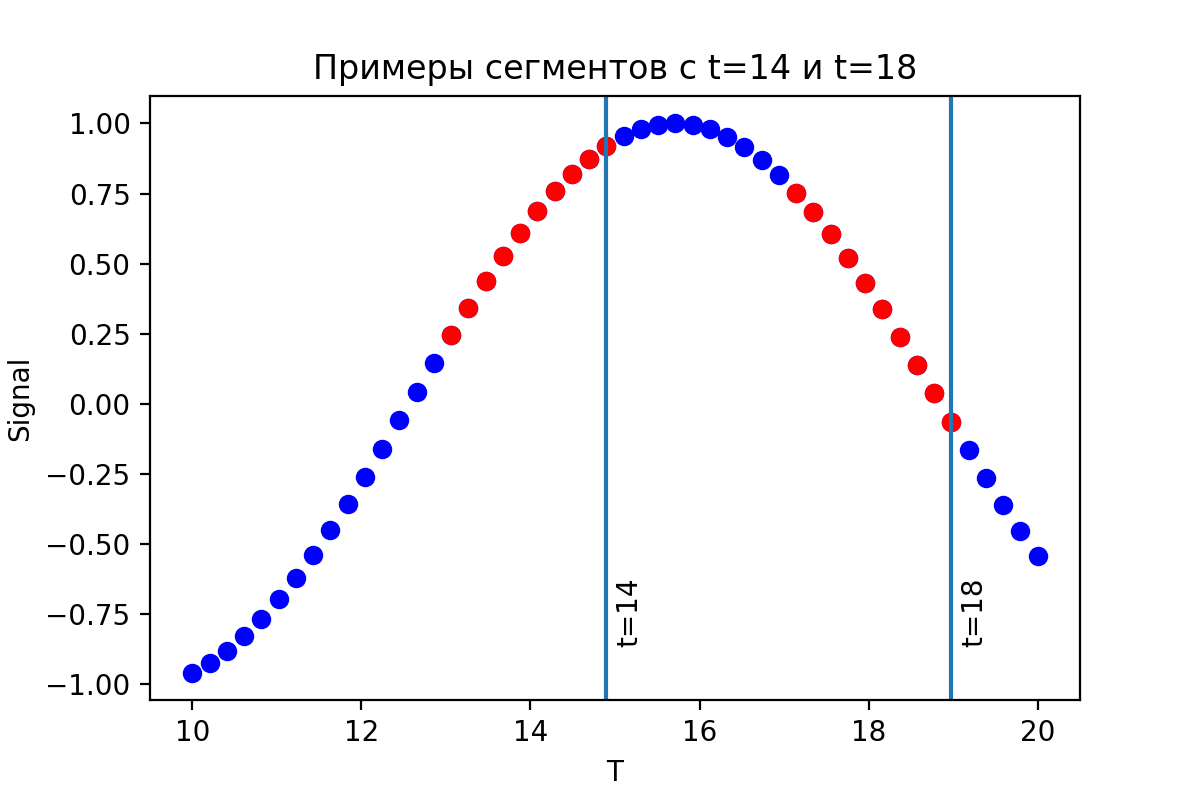
\includegraphics[width=0.5\textwidth]{../pics/segment_def.png}
\end{figure}

Необходимо восстановить зависимость $y = f(x), f: X \to \{1, 2, \ldots K\}$.
Для этого задана обучающая выборка

$$
\mathfrak{D} = \{ (x_i, y_i) \}_{i=1}^l, \;\;\; y_i \in \{1, 2, \ldots K\}
$$

а также функция потерь (multinomial log-loss)

\begin{equation} \label{init_logloss}
L(f(x_i), y) = \sum_{i=1}^l\sum_{k=1}^K [y_i = k]\log P(y_i = k| x_i, \theta)
\end{equation}

Таким образом мы решаем задачу оптимизации

$$
\hat{\theta} = \arg\min_{\theta \in \Theta} \sum_{i = 1}^l L(f(x_i), y_i)
$$

\subsection{Комбинированное признаковое описание}

Пусть $H$ --- множество функций вида
$h: X \to \R^m$, где $m = m(g)$, то есть это множество отображений
пространства объектов сложной структуры в пространство действительных чисел
некоторой размерности (для каждой функции размерность может быть своя). В
$G$ могут лежать, например

\begin{itemize}
    \item Множество моделей локальной аппроксимации сигнала
    \item Множество статистик
    \item Множество экспертных оценок каждого из сложных объектов
\end{itemize}

Возьмем конечный поднабор этих функций
$$
g = [h_1\ldots h_k], \{h_1\ldots h_k\} \subset H
$$

Обозначим сумму размерностей образов функций из набора как

$$
n_g \triangleq \mathrm{dim}(\mathrm{Im}(h_1)) +
\mathrm{dim}(\mathrm{Im}(h_2)) + \ldots +
\mathrm{dim}(\mathrm{Im}(h_k))
$$

Тогда $g$ индуцирует отображение $g: X \to Z \subset \R^{n_g}$,
причем в векторах образа первые $\mathrm{dim}(\mathrm{Im}(h_1))$ компонент соответствуют
образу $g_1$, следующие $\mathrm{dim}(\mathrm{Im}(h_2))$ соответствуют $h_2$
и так далее. $Z$ называется \textit{признаковым пространством}
объектов сложной структуры $X$. Тогда, мы можем искать $f$ в семействе
суперпозиций $a(g(\cdot), \gamma)$, где

$$
X \xrightarrow{h} Z \xrightarrow{a} Y
$$

\begin{itemize}
    \item $g$ --- это признаковое отображение
    \item $a(\cdot, \gamma)$ --- параметрическое отображение $Z$ в $\{1, 2, \ldots K\}$,
    которое соответствует некоторому алгоритму машинного обучения,
    параметризованного вектором гиперпараметров $\gamma$.
\end{itemize}

% Для отображения из параметрического пространства задана функция ошибки
% $L(h(g(s_i), \gamma), y_i)$, тогда задача разбивается на два этапа:
В таком подходе функция потерь \ref{init_logloss} теперь определена
на отображении $a$, то есть

$$
L(f(x), y) = L(a(g(x), \gamma), y)
$$

Итак, задача решается следующим образом:

\begin{itemize}
    \item Поиск и вычисление отображения $X = \{g(\{s_i\}_{i=1}^l), y_i)\}$.
    \item Определение оптимальных парметров $\gamma$ в задаче оптимизации
    $$
    \hat{\gamma} = \arg\min_{\gamma} \sum_{i=1}^{l}L(h(x_i, \gamma), y_i)
    $$
\end{itemize}

Основное допущение, принимаемое в данном методе является допущение о том, что
выборка в признаковом пространстве объектов является простой. В данной работе
мы рассматриваем, для каких признаковых пространств это допущение справедливо,
а также предлагаем способы построения таких выборок.

\section{Построение признакового пространства}

В качестве элементов из пространсва функций $H$ мы будем использовать
локально-аппроксимирующие модели сегментов.

$$
g(w, x) \in X, \text{ где }w \in \R^{n_g}
$$

Тогда параметры настроенной модели будут являться образом отображения $h$

$$
h(x) = \arg\min_{w \in \R^{n_g}} \rho(g(w, x), x)
$$

\subsection{Локально-аппроксимирующие модели}

\subsubsection{SEMOR}

Пусть наряду с сегментом $x$ мы имеем некоторый временной $p$, который содержит
меньшее число элементов. Модель предполагает, что изгиб временного ряда $p$ повторяет
форму $x$, поэтому мы аппроксимируем временной ряд $x$ сегментом $p$.

\begin{figure}[ht]
    \caption{Иллюстрация параметров метора SEMOR.}
    \centering
      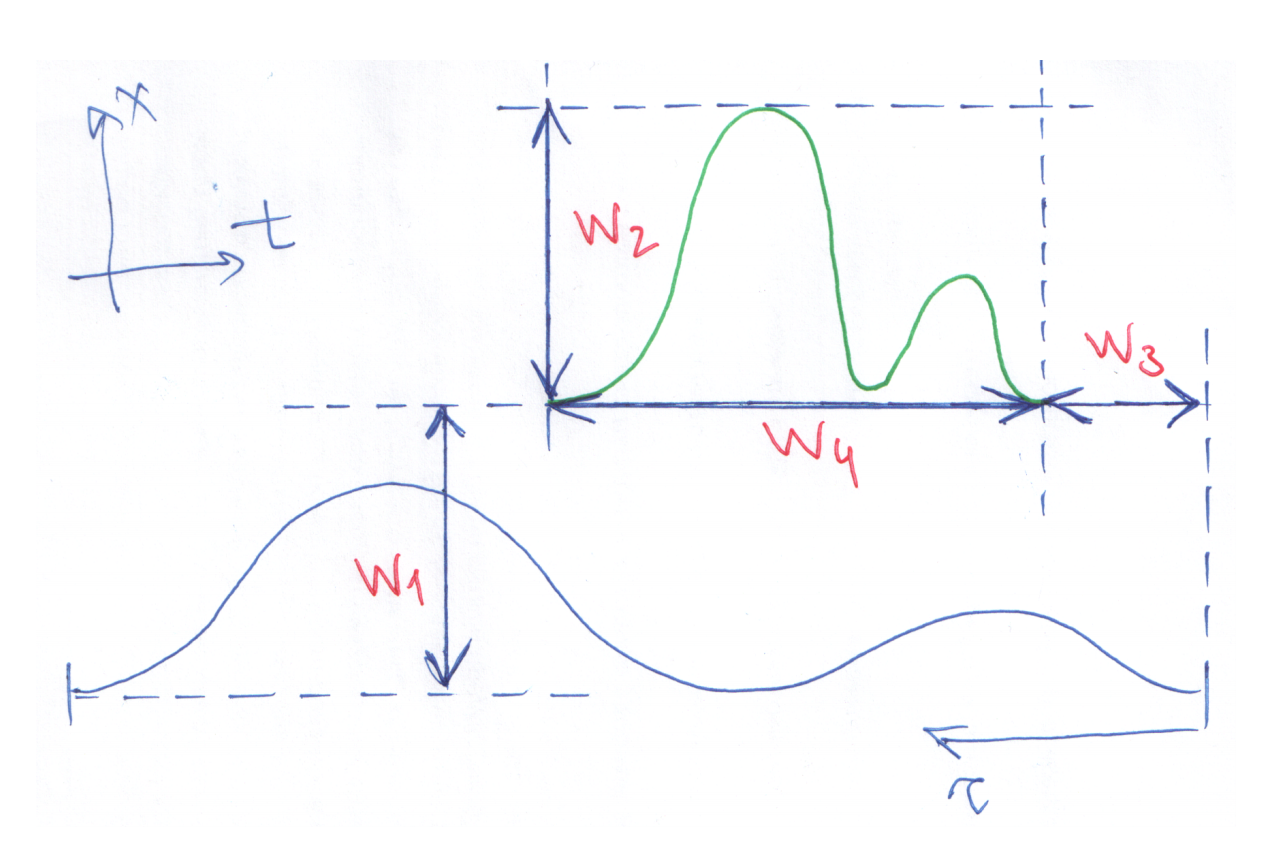
\includegraphics[width=0.5\textwidth]{../pics/semor_illustration.png}
\end{figure}

$$
w = [w_1, w_2, w_3, w_4]
$$

Модель Self-Modeling Regression описывается следующим выражением

$$
g(x, w) = w_1 + w_2 p(w_3 + w_4t)
$$

Где в общем случае $p$ --- функция формы, однако в частном случае это может
быть заранее заданный временной ряд. Параметры $w_1, w_2$ находятся шагом двухпараметрической
линейной регрессии, $w_3, w_4$ получаются минимизацией DTW, где из наклона
пути, результирующего в minimum edit distance мы получаем $w_4$, а $w_3$ — это
смещение этой прямой относительно нуля. Следуя приведенной схеме мы получаем
следующие оптимальные веса

$$
w_{\text{SEMOR}} = [\hat{w_1}, \hat{w_2}, \hat{w_3}, \hat{w_4}]
$$

\subsubsection{AR-авторегрессия}

Является моделью авторегрессии порядка $m$.

$$
g_{\text{AR}}(w, x) = [\hat{x_1} \ldots \hat{x_n}], \text{ где }
\hat{x}_i = \begin{cases}
    x_k & \text{ при } k \in [1, m] \\
    w_0 + \sum_{i=1}^m w_i x_{k - i} & \text{ при } k \in [m + 1, n]
\end{cases}
$$

Оптимальные веса $w$ определяются минимизацией некоторой функции ошибки, например
MSE

$$
w_{\text{AR}} = \arg\min_{w \in \R^m} \sum_{i=1}^{n}\norm{x_i - \hat{x_i}}^2
$$

\subsubsection{Фурье-модель}

С помощью эмбеддинга построим траекторную матрицу $S$ для сегмента $x \in \R^n$

$$
S = \begin{pmatrix}
x_1 & x_2 & \dots & x_m \\
x_2 & x_3 & \dots & x_{m + 1} \\
\vdots & \vdots & \ddots & \vdots \\
x_{n - m + 1} & x_{n - m + 2} & \dots & x_n
\end{pmatrix}
$$

Каждая следующая строка траекторной матрицы $S$ получается сдвиганием окна
длины $m$ в сегменте на единицу. $m$ --- единственный параметр SSE.
Применяем сингулярное разложение к матрице $X^\intercal X$

$$
X^\intercal X = VHV^\intercal
$$

Где $H = \mathrm{diag}(\lambda_1\ldots \lambda_m)$ --- диагональная матрица собственных значений.
Вектор, образованный этими собственными значениями используются в качестве
признакового описания сегмента $x$.

$$
w_{\text{SSA}} = [\lambda_1 \ldots \lambda_m]
$$

\subsubsection{Вейвлет-модель}

В качестве аппроксимирующей модели сегмента берем обратное дискретное
преобразование Фурье,
то есть признаковым описанием сегмента является прямое дискретное преобразование
Фурье.
$$
    w_{2j} = \mathrm{Re} \sum_{k=1}^{n} x_k \exp\brs{-\frac{2\pi i}{n}kj}, j=1\ldots n
$$
$$
    w_{2j + 1} = \mathrm{Im} \sum_{k=1}^{n} x_k \exp\brs{-\frac{2\pi i}{n}kj}, j=1\ldots n
$$
$$
w_{\text{FFT}} = \sbrs{w_1\ldots w_{2n}}\in \R^{2n}
$$


% %%%%%%%%%%%%%%%%%%%%%%%%%%%%%%%%%%%%%%%%%%%%%%%%%%%%%%%%%%%%%%%%%%%%%%%%%%%%%%
% \newpage
% \section{Метод частных наименьших квадратов (PLS)}
% %%%%%%%%%%%%%%%%%%%%%%%%%%%%%%%%%%%%%%%%%%%%%%%%%%%%%%%%%%%%%%%%%%%%%%%%%%%%%%
% Идея метода частных наименьших квадратов состоит в том, чтобы перейти в пространство меньшей размерности с сохранением ковариации между признаками и ответами. Матрица плана $\bX$ и матрица ответов $\bY$ проецируются на пространство меньшей размерности $m \times l$ так, что ковариация между новыми признаками и ответами максимальна:
% \begin{equation}
% \label{pls_x_y}
%     \bX = \bT \bP^{\T} + \bE,\\
%     \bY = \bU \bQ^{\T} + \bF
% \end{equation}
% $\bT \in \mathbb{R}^{m \times l},\ \bU \in \mathbb{R}^{m \times l}$~--- значения признаков и ответов в спроектированном пространстве. $\bP \in \mathbb{R}^{n \times l},\ \bQ \in \mathbb{R}^{r \times l}$~--- матрицы перехода из нового пространства в старое. $\bE\in \mathbb{R}^{m \times n},\ \bF \in \mathbb{R}^{m \times n}$~--- матрицы невязок.
% Так как ковариация между новыми признаками и ответами максимальна, то можно строить регрессионную модель в пространстве меньшей размерности с сохранением точности прогноза. Параметр метода частных наименьших квадратов $l \in \mathbb{N}$ определяет размерность этого пространства. Отбор признаков осуществляется в виде замены исходных признаков $[\bchi_1, \dots, \bchi_n]$ на $l$ новых признаков~--- линейные комбинации исходных признаков.


% Чтобы получить модель регрессии, связывающую $\bY$ и $\bX$, сначала находятся параметры $\beta_i$ такие, что $\bu_i = \bt_i \beta_i, \ i \in \{1, \dots, l\}$.
% Подставляя параметры в модель~(\ref{pls_x_y}), получаем
% $$
%     \bY = \bU\bQ^{\T} = \bT \text{diag}(\boldsymbol{\beta}) \bQ^{\T} = \bX \bTheta.
% $$

% Псевдокод метода PLSR приведен в алгоритме~\ref{PLSR_pseudo}. Из сохраненных на каждом из $l$ шагов значений $\mathbf{t}$, $\mathbf{u}$, $\mathbf{p}$, $\mathbf{q}$ формируются матрицы $\mathbf{T}$, $\mathbf{U}$, $\mathbf{P}$, $\mathbf{Q}$ соответственно.
% \begin{center}
% \begin{algorithm}[h]
% \caption{Алгоритм PLSR}
%     \label{PLSR_pseudo}
% \begin{algorithmic}[1]
% \REQUIRE $\bX, \bY, l$;
% \ENSURE $\bT, \bU, \bP, \bQ$;
% \STATE инициализировать $\bu := \by_1$ (вектор матрицы $\bY$)
% \FOR{$i=1,\dots, l$}
%   \REPEAT
%     \STATE $\bw := \bX^{\T} \bu / (\bu^{\T} \bu)$
%     \STATE нормировать $\bw$: $\| \bw \| = 1$
%     \STATE $\mathbf{t} := \bX \bw$
%     \STATE $\bc := \bY^{\T} \bt / (\bt^{\T} \bt)$
%     \STATE нормировать $\bc$:  $\| \bc \| = 1$
%     \STATE $\bu := \bY \bc$
%   \UNTIL{$\bt$ не перестанет меняться}
%   \STATE сохранить $\bt$, $\bu$, $\bc$
%   \STATE $\bp := \bX^{\T}\bt/(\bt^{\T}\bt),\ \bq := \bY^{\T}\bu/(\bu^{\T}\bu)$
%   \STATE регрессия ($\bu$ на $\bt$): $\beta := \bu^{\T} \bt / (\bt^{\T} \bt)$
%   \STATE $\bX := \bX - \bt\bt^{\T}\bX/(\bt^{\T}\bt)$
%   \STATE $\bY := \bY - \beta\bt\bc^{\T}$
% \ENDFOR
% \end{algorithmic}
% \end{algorithm}
% \end{center}

% Размеры векторов в алгоритме можно изобразить следующим образом:

% \tikzstyle{sensor_x}=[draw, fill=blue!0, text width=4em,
%     text centered, minimum height=5em]
% \tikzstyle{sensor_y}=[draw, fill=blue!0, text width=2.7em,
%     text centered, minimum height=5em]


% \def\blockdist{2.3}
% \def\edgedist{2.5}

% % \vspace{1cm}
% \hspace{1cm}
% \begin{figure}[H]
% \centering
% \begin{tikzpicture}
%     \node (x) [sensor_x]  {$\bX$};
%     \path (x.east)+(4,0) node (y) [sensor_y] {$\bY$};

%     %X
%     \path [draw, -] +(1.2, 0.9) -- node [right] {$\bt$}
%       +(1.2,-0.9);
%     \path [draw, -] +(0.8, -2) -- node [left of=2] {$\bp^{\T}$}
%       +(-0.8, -2);
%     \path [draw, -] +(0.8, -1.5) -- node [left of=2] {$\bw^{\T}$}
%       +(-0.8, -1.5);
%     %Y
%     \path [draw, -] +(3.85, 0.9) -- node [left] {$\bu$}
%       +(3.85,-0.9);
%     \path [draw, -] +(4.2, -2) -- node [left of=-1.3] {$\bq^{\T}$}
%       +(5.4, -2);
%     \path [draw, -] +(4.2, -1.5) -- node [left of=-1.3] {$\bc^{\T}$}
%       +(5.4, -1.5);
% \end{tikzpicture}
% \caption{Размерности векторов в алгоритме PLS}
% \end{figure}
% % \begin{center}
% % \begin{algorithm}
% % \begin{algorithmic}[1]
% % \REQUIRE $\mathbf{X}, \mathbf{Y}, l$;
% % \ENSURE $\mathbf{T}, \mathbf{U}, \mathbf{P}, \mathbf{Q}$;
% % \FOR{$i=1,\dots,l$}
% %   \STATE $\mathbf{u} := \mathbf{y}_j$ для произвольного $j$
% %   \REPEAT
% %     \STATE $\mathbf{p := \dfrac{X^{\mathsf{T}}u}{\left\|X^{\mathsf{T}}u \right\|}}$
% %     \STATE $\mathbf{t := Xp}$
% %     \STATE $\mathbf{q := \dfrac{Y^{\mathsf{T}}t}{\left\|Y^{\mathsf{T}}t \right\|}} $
% %     \STATE $\mathbf{u := Yq}$
% %   \UNTIL{$\mathbf{t}$ не перестанет меняться}
% %   \STATE сохранить $\mathbf{t}$, $\mathbf{u}$, $\mathbf{p}$, $\mathbf{q}$
% %   \STATE  $\mathbf{X := X - tp^{\T}}$
% %   \STATE $\mathbf{Y := Y - uq^{\T}}$
% % \ENDFOR
% % \end{algorithmic}
% % \end{algorithm}
% % \end{center}



% В \cite{ng2013simple} показано, что вектора $\bw$ и $\bc$ во внутреннем цикле максимизируют ковариацию между новыми признаками и матрицей ответов:

% $$
%         [\text{cov} (\bt, \bu)]^2 = [\text{cov} (\bX \bw, \bY \bc)]^2 = \max\limits_{\|\bs\|=1, \|\br\|=1} [\text{cov} (\bX \bs, \bY \br)]^2,
% $$
% где $\text{cov} (\bt, \bu) = \bt^{\T} \bu / n$ означает выборочную ковариацию.

% % \begin{equation}
% % \mathbf{p} = \argmax_{\left\| \mathbf{w} \right\| = 1} \text{Var}(\mathbf{Xw})  {\left( \text{Corr}\left(\mathbf{Y}, \mathbf{Xw}\right)\right)}^\mathsf{T} {\left( \text{Corr}\left(\mathbf{Y}, \mathbf{Xw}\right)\right)}
% % \end{equation}

% %%%%%%%%%%%%%%%%%%%%%%%%%%%%%%%%%%%%%%%%%%%%%%%%%%%%%%%%%%%%%%%%%%%%%%%%%%%%%%
% \newpage
% \section{Модификация метода частных наименьших квадратов (cnlPLS)}
% %%%%%%%%%%%%%%%%%%%%%%%%%%%%%%%%%%%%%%%%%%%%%%%%%%%%%%%%%%%%%%%%%%%%%%%%%%%%%%
%     Предлагается провести модификацию алгоритма PLS: совершить криволинейное и нелинейное преобразования пространства целевой переменной  и независимой переменной для учета мультиколлинеарности между сигналами в разные моменты времени. Схема модифицированного алгоритма представлена на рис.~4.


% \tikzstyle{sensor_x}=[draw, fill=blue!0, text width=4em,
%     text centered, minimum height=5em]
% \tikzstyle{sensor_y}=[draw, fill=blue!0, text width=2.7em,
%     text centered, minimum height=5em]
% \begin{figure}[H]
% \label{scheme_cnlPLS}
% \centering
% {\footnotesize
% \def\blockdist{2.3}
% \def\edgedist{2.5}
% \vspace{1cm}
% \hspace{1cm}
% \begin{tikzpicture}
%     \node (x) [sensor_x]  {$\bX$};
%     \path (x.south)+(0,-2) node (tilde_x) [sensor_x] {$\tilde \bX$};
%     \path (x.east)+(4,0) node (y) [sensor_y] {$\bY$};
%     \path (y.south)+(0,-2) node (tilde_y) [sensor_y] {$\tilde \bY$};
%     \path (tilde_x.south)+(0,-0.8) node (x_form) {$\tilde \bX = \bT \bP^{T} + \bE$};
%     \path (tilde_y.south)+(0.4,-0.8) node (y_form) {$\tilde \bY = \bU \bQ^{\T} + \bM$};
%     \path (tilde_x.south)+(2.5,-1.3) node (u_form) {$\bU = \bT \bD + \bZ$};


%     \path [draw, ->] (x.south) -- node [right] {$f_x(\bX, \bv_x)$}
%         (tilde_x.north);
%     \path [draw, ->] (y.south) -- node [right] {$f_y(\bY, \bv_y)$}
%         (tilde_y.north);
%     %tilde X
%     \path [draw, -] +(1,-2) -- node [right] {$\bt$}
%       +(1,-3.7);
%     \path [draw, -] +(0.8,-3.9) -- node [below] {$\bp$}
%       +(-0.8,-3.9);
%     %tilde Y
%     \path [draw, -] +(4.05,-2) -- node [left] {$\bu$}
%       +(4.05,-3.7);
%     \path [draw, -] +(4.2,-3.9) -- node [below] {$\bq$}
%       +(5.4,-3.9);

%     \path [draw, ->] +(0.79,-3.77) -- node [above] {$\bw$}
%       +(2.31,-4.8);
%     \path [draw, ->] +(4.21,-3.77) -- node [above] {$\bc$}
%       +(1.9,-4.8);
% \end{tikzpicture}
% }
% \caption{Схема модифицированного метода частных наименьших квадратов}
% \end{figure}
% %%%%%%%%%%%%%%%%%%%%%%%%%%%%%%%%%%%%%%%%%%%%%%%%%%%%%%%%%%%%%%%%%%%%%%%%%%%%%%
% \subsection{Преобразование зависимой переменной}
% %%%%%%%%%%%%%%%%%%%%%%%%%%%%%%%%%%%%%%%%%%%%%%%%%%%%%%%%%%%%%%%%%%%%%%%%%%%%%%

%     Рассматриваются следующие преобразования пространства зависимой переменной $\bY$:
%     \begin{itemize}
%     \item криволинейное с вектором параметров $\bv$ (примеры преобразований представлены в таб.~\ref{table_functions})
%     \begin{equation}
%     \label{transf_y}
%         \breve \bY = g (\bY, \bv),
%     \end{equation}
%     \item нелинейное непараметрическое преобразование
%     \begin{equation*}
%         \hat \bY = h (\bY),
%     \end{equation*}
%     \item суперпозиция преобразований   $
%     \begin{diagram}
%     \node{\bY}
%     \arrow{e,t}{g(\bY, \bv)}
%     \node{\breve \bY}
%     \arrow{e,t}{h(\breve \bY)}
%     \node{\tilde \bY}
%     \end{diagram}
%     $
%     \begin{equation*}
%         \tilde \bY = h (\breve \bY) = h( g( \bY, \bv)) = f(\bY, \bv).
%     \end{equation*}

%     \end{itemize}


%     % $$
%     %     \begin{diagram}
%     %     \node{\bY}
%     %     \arrow{e,t}{g(\bY, \bv)}
%     %     \node{\breve \bY}
%     %     \arrow{e,t}{h(\breve \bY)}
%     %     \node{\tilde \bY}
%     %     \end{diagram}
%     %     $$

% % \begin{table}
% % \centering
% % \begin{tabular}{l|l|l|l|}
% % \cline{2-4}
% %   & \textbf{Функция}                                 & \textbf{Параметры} & \textbf{Обратная}                                             \\ \cline{2-4}
% % 1 & $g(x) = \sign(x)\exp(a)(\exp(b|x|) - 1$          & $a, b > 0$         & $g^{-1}(y) = \sign(y) \exp(-b)\log(|y| \exp(-a) + 1)$         \\ \cline{2-4}
% % 2 & $g(x) = \sign(x)\exp(a)(\exp(b\ln(1+ \,|x|) - 1$ & $a, b > 0$         & $g^{-1}(y) = \sign(y)\exp( \exp(-b)\log(|y| \exp(-a) + 1)-1)$ \\ \cline{2-4}
% % 3 & $g(x) = \sign(x)\exp(a)(\exp(b|x|^{1/2}) - 1$    & $a, b > 0$         & $g^{-1}(y) = \sign(y) (\exp(-b)\log(|y| \exp(-a) + 1))^2$     \\ \cline{2-4}
% % 4 & $g(x) = \sign(x)\exp(a)(\exp(b|x|^{1/3}) - 1$    & $a, b > 0$         & $g^{-1}(y) = \sign(y) (\exp(-b)\log(|y| \exp(-a) + 1))^3$     \\ \cline{2-4}
% % 5 & $g(x) = \sign(x)\exp(a)(\exp(b|x|^{1/4}) - 1$    & $a, b > 0$         & $g^{-1}(y) = \sign(y) (\exp(-b)\log(|y| \exp(-a) + 1))^4$     \\ \cline{2-4}
% % 6 & $g(x) = \sign(x)\exp(a)(\exp(b|x|^{2}) - 1$      & $a, b > 0$         & $g^{-1}(y) = \sign(y) (\exp(-b)\log(|y| \exp(-a) + 1))^{1/2}$ \\ \cline{2-4}
% % \end{tabular}
% % \caption{Криволинейные преобразования}
% % \label{table_functions}
% % \end{table}
% Криволинейные преобразования выбирались таким образом, чтобы функции преобразования удовлетворяли следующим условиям:
% \begin{itemize}
%     \item отображает множество действительных чисел во множество действительных чисел $g: \mathbb{R} \to \mathbb{R}$,
%     \item принимает нулевое значение в нуле $g(0) = 0$,
%     \item дифференцируется по параметрам,
%     \item является обратимой, то есть существует $g^{-1}$.
% \end{itemize}

% \begin{table}[]
% \centering
% \begin{tabular}{|l|l|l|}
% \hline
% \textbf{№} & \textbf{Функция}                                  & \textbf{Параметры} \\ \hline
% 1          & $g(x) = \sign(x)\exp(a)(\exp(b|x|) - 1)$          & $a, b > 0$         \\ \hline
% 2          & $g(x) = \sign(x)\exp(a)(\exp(b\ln(1+ \,|x|) - 1)$ & $a, b > 0$         \\ \hline
% 3          & $g(x) = \sign(x)\exp(a)(\exp(b|x|^{1/2}) - 1)$    & $a, b > 0$         \\ \hline
% 4          & $g(x) = \sign(x)\exp(a)(\exp(b|x|^{1/3}) - 1)$    & $a, b > 0$         \\ \hline
% 5          & $g(x) = \sign(x)\exp(a)(\exp(b|x|^{1/4}) - 1)$    & $a, b > 0$         \\ \hline
% 6          & $g(x) = \sign(x)\exp(a)(\exp(b|x|^{2}) - 1)$      & $a, b > 0$         \\ \hline
% \end{tabular}
% \caption{Криволинейные преобразования}
% \label{table_functions}
% \end{table}

%     Предлагается подход для обновления весов $\bv$, основаный на линеаризации функции преобразования. Разложим (\ref{transf_y}) в ряд Тейлора до второго порядка:
%     $$
%         \breve \by \approx \breve \by_{0} + \frac{\partial g}{\partial \bv} \Big|_{0} \Delta \bv,
%     $$
%     где $\breve \by_{0}$~--- это значение функции $g$ при известном значении переменной $\by$.
%     Для вычисления $\Delta \bv$ предложены следующие шаги. Рассматривается разница $\breve \by - \breve \by_{0} = \frac {\partial g_y}{\partial \bv_y} \Big|_{0} \Delta \bv$. Определется рассогласование $\be$
%     $$
%         \be = \breve \by - \breve \by_{0} = \frac {\partial g}{\partial \bv} \Big|_{0} \Delta \bv = \bJ_y \Delta \bv,
%     $$
%     где матрица $\bJ_y$ состоит из частных производных $\left\{\frac {\partial g}{\partial v_i}\Big|_{0} \right\}_{i=1}^N$, вычисленных при известном значении переменной $\by$. Далее $\Delta \bv$ вычисляется решением задачи регрессии рассогласования $\be$ так, что
%   \begin{equation}
%   \label{delta_v}
%     \Delta \bv  = (\bJ_y^{\T} \bJ_y)^{-1} \bJ_y^{\T} \be.
%   \end{equation}
% %%%%%%%%%%%%%%%%%%%%%%%%%%%%%%%%%%%%%%%%%%%%%%%%%%%%%%%%%%%%%%%%%%%%%%%%%%%%%%
% \subsection{Преобразование независимой переменной}
% %%%%%%%%%%%%%%%%%%%%%%%%%%%%%%%%%%%%%%%%%%%%%%%%%%%%%%%%%%%%%%%%%%%%%%%%%%%%%%
%     Аналогично преобразованию целевой переменной $\bY$, совершается преобразование зависимой переменной $\bX$ для учета мультиколлинеарности в признаковом пространстве.

%     Рассмотрим преобразования $\bX$
%     \begin{itemize}
%     \item криволинейное с вектором параметров $\bv$ (таб.~\ref{table_functions})
%     \begin{equation}
%     \label{transf_y}
%         \breve \bX = g (\bX, \bv),
%     \end{equation}
%     \item нелинейное непараметрическое преобразование
%     \begin{equation*}
%         \hat \bX = h (\bX),
%     \end{equation*}
%     \item суперпозиция преобразований
%     \begin{equation*}
%         \tilde \bX = h (\breve \bX) = h( g( \bX, \bv)) = f(\bX, \bv).
%     \end{equation*}
%     \end{itemize}

% %%%%%%%%%%%%%%%%%%%%%%%%%%%%%%%%%%%%%%%%%%%%%%%%%%%%%%%%%%%%%%%%%%%%%%%%%%%%%%
% \subsection{Алгоритм cnlPLSR}
% %%%%%%%%%%%%%%%%%%%%%%%%%%%%%%%%%%%%%%%%%%%%%%%%%%%%%%%%%%%%%%%%%%%%%%%%%%%%%%
%     В данном разделе представлен модифицированный метод PLSR, содержащий шаги преобразования целевой переменной. Аналогично методу PLSR (алгоритм~\ref{PLSR_pseudo}), алгоритм \ref{cnlPLSR_pseudo} начинается с инициализации вектора $\bu$, а обновления весов преобразования считается с помощью рассогласования $\be$ для вектора $\bu$, вычисленного в цикле и на предыдущей итерации.
%     \vspace{-0.5cm}
% \begin{center}
% \begin{algorithm}[H]
% \caption{Алгоритм cnlPLSR}
%     \label{cnlPLSR_pseudo}
% \begin{algorithmic}[1]
% \REQUIRE $\bX, \bY, l$;
% \ENSURE $\bT, \bU, \bP, \bQ$;
% \STATE инициализировать $\bv$
% \STATE определить $\bu_0$ как вектор преобразования $f(\bY, \bv)$
% \FOR{$i=1,\dots, l$}
%   \REPEAT
%     \STATE $\bw := \bX^{\T} \bu_0 / (\bu_0^{\T} \bu_0)$
%     \STATE нормировать $\bw$: $\| \bw \| = 1$
%     \STATE $\mathbf{t} := \bX \bw$
%     \STATE $\tilde \bY = f(\bY, \bv)$
%     \STATE $\bc := \tilde \bY^{\T} \bt / (\bt^{\T} \bt)$
%     \STATE нормировать $\bc$: $\| \bc \| = 1$
%     \STATE $\bu := \tilde \bY \bc$
%     \STATE $\be := \bu - \bu_0$
%     \STATE $\bJ := \partial \bu / \partial \bv$
%     \STATE $\Delta \bv = (\bJ^{\T} \bJ)^{-1} \bJ^{\T} \be$
%     \STATE $\bv := \bv + \Delta \bv,\ \|\bv\| = 1$
%     \STATE $\bu_0 := \bu$
%   \UNTIL{$\bt$ не перестанет меняться}
%   \STATE сохранить $\bt$, $\bu$, $\bc$
%   \STATE вычислить $\tilde \bY$
%   \STATE $\bp := \bX^{\T}\bt/(\bt^{\T}\bt),\ \bq := \tilde \bY^{\T}\bu/(\bu^{\T}\bu)$
%   \STATE регрессия ($\bu$ на $\bt$): $\beta := \bu^{\T} \bt / (\bt^{\T} \bt)$
%   \STATE $\bX := \bX - \bt\bt^{\T}\bX/(\bt^{\T}\bt)$
%   \STATE $\tilde{\bY} := \tilde \bY - \beta\bt\bc^{\T}$
%   \STATE вычислить $\bY$ с помощью обратного преобразования $f^{-1}(\tilde \bY, \bv)$
% \ENDFOR
% \end{algorithmic}
% \end{algorithm}
% \end{center}

% %%%%%%%%%%%%%%%%%%%%%%%%%%%%%%%%%%%%%%%%%%%%%%%%%%%%%%%%%%%%%%%%%%%%%%%%%%%%%%
% \newpage
% \section{Вычислительный эксперимент}
% %%%%%%%%%%%%%%%%%%%%%%%%%%%%%%%%%%%%%%%%%%%%%%%%%%%%%%%%%%%%%%%%%%%%%%%%%%%%%%
% В рамках вычислительного эксперимента строится прогноз временных рядов. В ходе эксперимента сравниваются методы PLSR, нелинейных автоэнкодеров и cnlPLS. Сравнение проводится на реальных данных объемов потребления электроэнергии в Польше.

% Вычислительный эксперимент, продемонстрированный в этом разделе, основан на данных электроэнергии. Данные состоят из временного ряда польских электрических нагрузок и временных рядов погоды в Варшаве (долгота: 21,25, широта: 52,30, высота над уровнем моря: 94). Временные ряды энергии состоят из почасовых записей (всего 52512 наблюдений), а погодные измерения проводились раз в день и содержат 2188 наблюдений. Многомасштабные временные ряды соответствуют периоду 1999-2004 годов. Результаты, полученные с этим набором данных, являются иллюстрацией предлагаемых методов, поскольку данные содержат многомасштабне временные ряды, имеющие различный характер.

% Примеры работы алгоритма приведены на рис.~\ref{fig:forecast}. Метод успешно делает краткосрочный прогноз (до 10 дней). С увеличением горизонта прогнозирования предсказание смещается.

% \begin{figure}[H]
%     \centering
%     \begin{subfigure}[b]{0.3\textwidth}
%         \includegraphics[width=\textwidth]{oneday.png}
%     \end{subfigure}
%     \begin{subfigure}[b]{0.3\textwidth}
%         \includegraphics[width=\textwidth]{twodays.png}
%     \end{subfigure}
%     \begin{subfigure}[b]{0.3\textwidth}
%         \includegraphics[width=\textwidth]{fivedays.png}
%     \end{subfigure}
%     \begin{subfigure}[b]{0.3\textwidth}
%         \includegraphics[width=\textwidth]{tendays.png}
%     \end{subfigure}
%     \begin{subfigure}[b]{0.3\textwidth}
%         \includegraphics[width=\textwidth]{twentydays.png}
%     \end{subfigure}
%     \begin{subfigure}[b]{0.3\textwidth}
%         \includegraphics[width=\textwidth]{month.png}
%     \end{subfigure}
%     \caption{Прогнозирование базового алгоритма на 1, 2, 5, 10, 20, 30 дней}
%     \label{fig:forecast}
% \end{figure}

% Результаты вычислительного эксперимента для предложенного модифицированного алгоритма cnlPLS представлены на рис.~\ref{fig:animals}. На графиках изображены сглаженные зависимости ошибки MSE от числа компонент в алгоритме для разных функций. Из графиков видно, что для функций $(a)-(e)$ ошибка при увеличении числа компонент падает, затем колеблется, слабо меняясь. Ошибка алгоритма с функцией $(f)$ увеличивается при увеличении числа компонент. Это означает, что преобразование, выполненное в пространстве целевой переменной с помощью функции $(f)$, плохо описывает зависимость. Меньшую ошибку имеют функции, растущие медленнее, а именно $(d)$ и $(e)$.

% \begin{figure}
%     \centering
%     \begin{subfigure}[b]{0.4\textwidth}
%         \includegraphics[width=\textwidth]{exp_abs_x.png}
%         \caption{$g(x) = \sign(x) e^a(\exp(b|x|) - 1)$}
%         \label{fig:exp_abs_x}
%     \end{subfigure}
%     ~ %add desired spacing between images, e. g. ~, \quad, \qquad, \hfill etc.
%       %(or a blank line to force the subfigure onto a new line)
%     \begin{subfigure}[b]{0.4\textwidth}
%         \includegraphics[width=\textwidth]{exp_log_x.png}
%         \caption{$g(x) = \sign(x)e^a(\exp(b\ln(1+ \,|x|) - 1)$}
%         \label{fig:exp_log_x}
%     \end{subfigure}
%     ~ %add desired spacing between images, e. g. ~, \quad, \qquad, \hfill etc.
%     %(or a blank line to force the subfigure onto a new line)
%     \begin{subfigure}[b]{0.4\textwidth}
%         \includegraphics[width=\textwidth]{exp_x_1_2.png}
%         \caption{$g(x) = \sign(x)e^a(\exp(b|x|^{1/2}) - 1)$}
%         \label{fig:exp_x_1_2}
%     \end{subfigure}
%     \begin{subfigure}[b]{0.4\textwidth}
%         \includegraphics[width=\textwidth]{exp_x_1_3.png}
%         \caption{$g(x) = \sign(x)e^a(\exp(b|x|^{1/3}) - 1)$ }
%         \label{fig:exp_x_1_3}
%     \end{subfigure}
%     ~ %add desired spacing between images, e. g. ~, \quad, \qquad, \hfill etc.
%       %(or a blank line to force the subfigure onto a new line)
%     \begin{subfigure}[b]{0.4\textwidth}
%         \includegraphics[width=\textwidth]{exp_x_1_4.png}
%         \caption{$g(x) = \sign(x)e^a(\exp(b|x|^{1/4}) - 1)$}
%         \label{fig:exp_x_1_4}
%     \end{subfigure}
%     ~ %add desired spacing between images, e. g. ~, \quad, \qquad, \hfill etc.
%     %(or a blank line to force the subfigure onto a new line)
%     \begin{subfigure}[b]{0.4\textwidth}
%         \includegraphics[width=\textwidth]{exp_x_2.png}
%         \caption{$g(x) = \sign(x)e^a(\exp(b|x|^{2}) - 1)$}
%         \label{fig:exp_x_2}
%     \end{subfigure}
%     \caption{Зависимость ошибки от числа компонент в алгоритме cnlPLS для разных функций}\label{fig:animals}
% \end{figure}

% В табл.~\ref{results} продемонстрировано увеличение точности прогнозивания при использовании криволинейного преобразования в пространстве зависимой переменной, но увеличение точности в пределах погрешности алгоритма (0.0005-0.0010). Функции с быстрым ростом не позволяют описать зависимость.
% \begin{table}[]
% \centering
% \begin{tabular}{|l|l|l|l|l|}
% \hline
% \textbf{Алгоритм}                                                                                  & \textbf{N=3}     & \textbf{N=5}     & \textbf{N=10}    & \textbf{N=20}    \\ \hline
% PLS                                                                                                & 0,00404          & 0,00337          & \textbf{0,00151} & 0,00135          \\ \hline
% \begin{tabular}[c]{@{}l@{}}cnlPLS\\ $g(x) = \sign(x)\exp(a)(\exp(b|x|) - 1)$\end{tabular}          & 0.00529          & 0.00514          & 0.00536          & 0.00506          \\ \hline
% \begin{tabular}[c]{@{}l@{}}cnlPLS\\ $g(x) = \sign(x)\exp(a)(\exp(b\ln(1+ \,|x|) - 1)$\end{tabular} & 0.00362          & 0.00386          & 0.00326          & 0.00317          \\ \hline
% \begin{tabular}[c]{@{}l@{}}cnlPLS\\ $g(x) = \sign(x)\exp(a)(\exp(b|x|^{1/2}) - 1)$\end{tabular}    & 0.00272          & 0.00236          & 0.00287          & \textbf{0.00128} \\ \hline
% \begin{tabular}[c]{@{}l@{}}cnlPLS\\ $g(x) = \sign(x)\exp(a)(\exp(b|x|^{1/3}) - 1)$\end{tabular}    & \textbf{0.00241} & \textbf{0.00233} & 0.00221          & 0.00173          \\ \hline
% \begin{tabular}[c]{@{}l@{}}cnlPLS\\ $g(x) = \sign(x)\exp(a)(\exp(b|x|^{1/4}) - 1)$\end{tabular}    & 0.00796          & 0.00768          & 0.00737          & 0.00803          \\ \hline
% \begin{tabular}[c]{@{}l@{}}cnlPLS\\ $g(x) = \sign(x)\exp(a)(\exp(b|x|^{2}) - 1)$\end{tabular}      & 0.00816          & 0.00798          & 0.00796          & 0.00775          \\ \hline
% \end{tabular}
% \caption{Значения ошибки MSE для разных чисел компонент и разных функций}
% \label{results}
% \end{table}

% %%%%%%%%%%%%%%%%%%%%%%%%%%%%%%%%%%%%%%%%%%%%%%%%%%%%%%%%%%%%%%%%%%%%%%%%%%%%%%
% \section{Заключение}
% В данной работе предложен новый подход к обнаружению зависимостей в пространстве зависимой переменной задачи прогнозирования временных рядов. Сравнивались результаты прогнозирования временных рядов, полученных с помощью метода частных наименьших квадратов и предложенной модификации. Проведен вычислительный эксперимент на реальных данных потребления электроэнергии в Варшаве. Построенная прогностическая модель показала высокое качество предсказания электрической нагрузки.
% %%%%%%%%%%%%%%%%%%%%%%%%%%%%%%%%%%%%%%%%%%%%%%%%%%%%%%%%%%%%%%%%%%%%%%%%%%%%%%
% %\section*{СПИСОК ЛИТЕРАТУРЫ}

%\bibliographystyle{gost71sv}
%\bibliography{MachLearn}
\newpage
\nocite{*}

\bibliographystyle{unsrt}
\bibliography{papers.bib}
% \begin{thebibliography}{00}


% \bibitem{uspenskiy15amctm}
%     Uspenskiy\;V., Vorontsov\;K., Tselykh\;V., Bunakov\;V.
%     Information Function of the Heart:
%     Discrete and Fuzzy Encoding of the ECG-Signal for Multidisease Diagnostic System.
%     In~\emph{Advanced Mathematical and Computational Tools in Metrology and Testing X, Series on Advances in Mathematics for Applied Sciences}. 2015. World Scientific. Singapore. Vol.\,86. Pp. 377--384.
% \end{thebibliography}





\end{document}
